\section{Design} % (fold)
\label{sec:design}
The main goal of the Realms system is to help in the creation of simple location-based applications using a configuration process and consists of the following two major components:
\begin{itemize}
	\item \emph{configuration manager} - empowers users with the possibility of augmenting a physical space with virtual properties and rules (we call it a realm). It also has the responsibility of holding the configured virtual spaces and guides the user-system interaction based on each user's context (location) information and possible virtual properties of the system (which can be applied in the user's context).
	\item \emph{mobile client} - collects relevant context data and intermediates the interaction between the users and the system
\end{itemize}

\noindent From a hardware perspective, the mobile client is meant to run on a mobile platform (i.e. such as Android, iOS etc.) enabled with the necessary technologies to collect location data (i.e. GPS, mobile network, wi-fi). Although most mobile devices running one of the required platforms support internet connection, we would like to note that this is a mandatory requirement. The realms server is intended to run on a stationary computer connected to the internet.
\\

\noindent There are two end user types which will use our system: the realm managers, which create realms using the realm configurator, and the realm users which interact with the realms using the provided mobile client. Actually, the mobile client users are end-users both to us and the realm managers: they are our end-users because they use the mobile client, that we provide, to connect to one of the realms, provided by realm managers. To make a clear distinction between the components each user type interacts with, we have illustrated a system usecase scenario in Figure \ref{fig.system_usecase}. From the usecase we can conclude that the realm managers connect through a web-based interface to the reams server which enables them to manage their realms, while the realm users connect to the realms server using the provided mobile application.
\begin{figure}
	\centering
	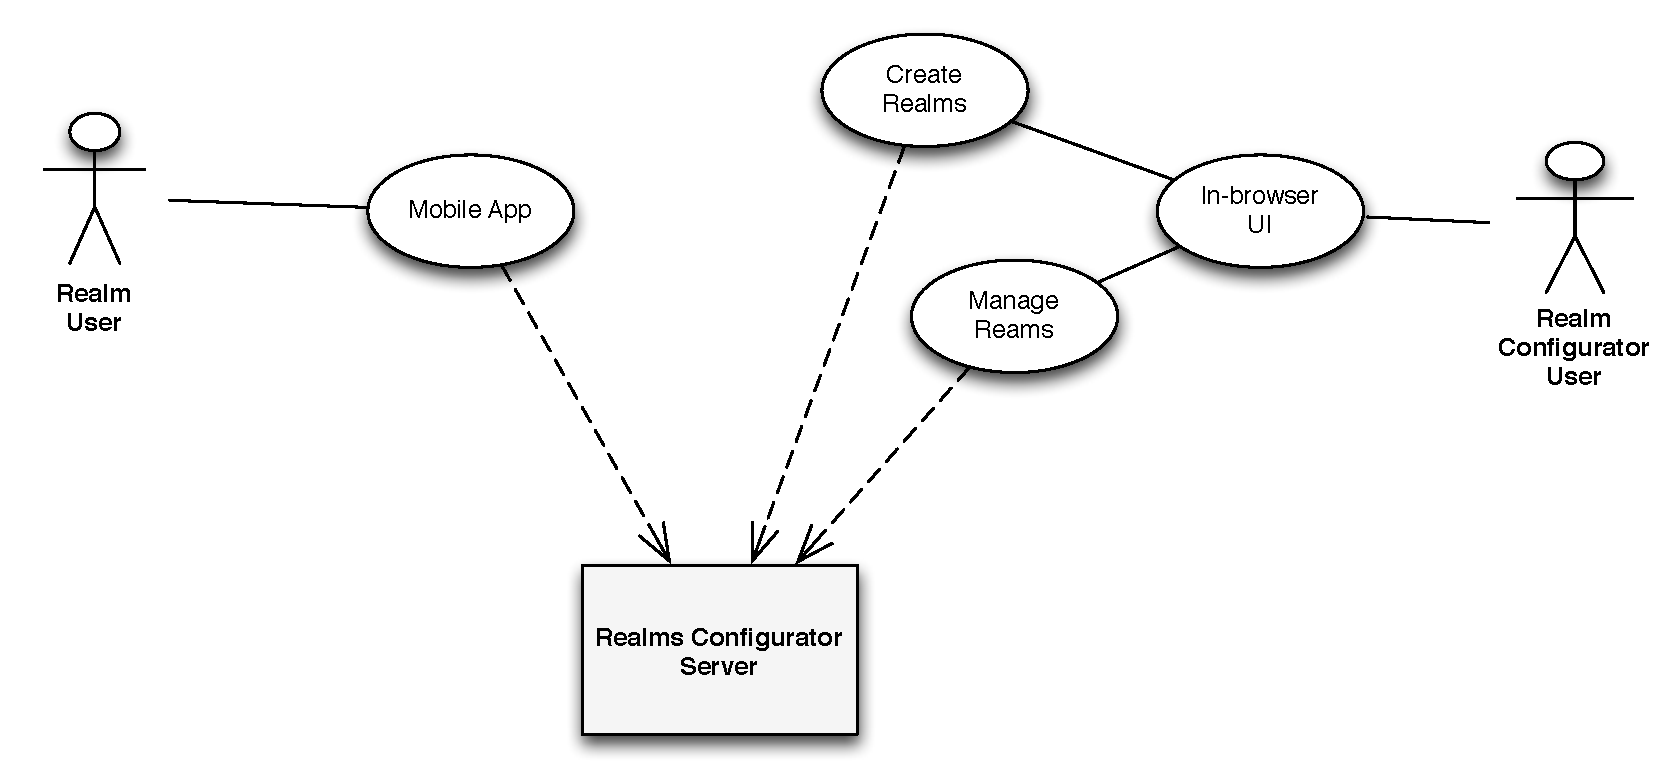
\includegraphics[width=1.0\linewidth]{fig/system_use_usecase}
	\caption{Realms system usecase scenario}
	\label{fig.system_usecase}
\end{figure}
\\

\\
\noindent Indoor positioning needs a lot more infrastructure than the one provided by GPS satellites which makes indoor locations hard to deal with. Hence, we consider indoor spaces to be out of scope for our system and the realms which a configuration manager will be able to create can be based only on outdoors spaces - we are excluding the possibility of indoors usage of the application and the mobile clients are meant to work only outdoors.
\\

\noindent The main advantage over similar system is that we empower users to create a ready-to-be-used location-based application without writing one line of code.
\\

\noindent The whole system is built around three main entities: \emph{location information}, \emph{virtual properties} and \emph{rules/decisions} to govern the data; hence, we are dealing with a data-driven system. Moreover,  the system is made up by a mobile client and a central infrastructure, the nature of the system being distributed. The natural choice to design such a system is to follow the client-server model \cite{Coulouris:2005}.
\\

\begin{figure}
	\centering
	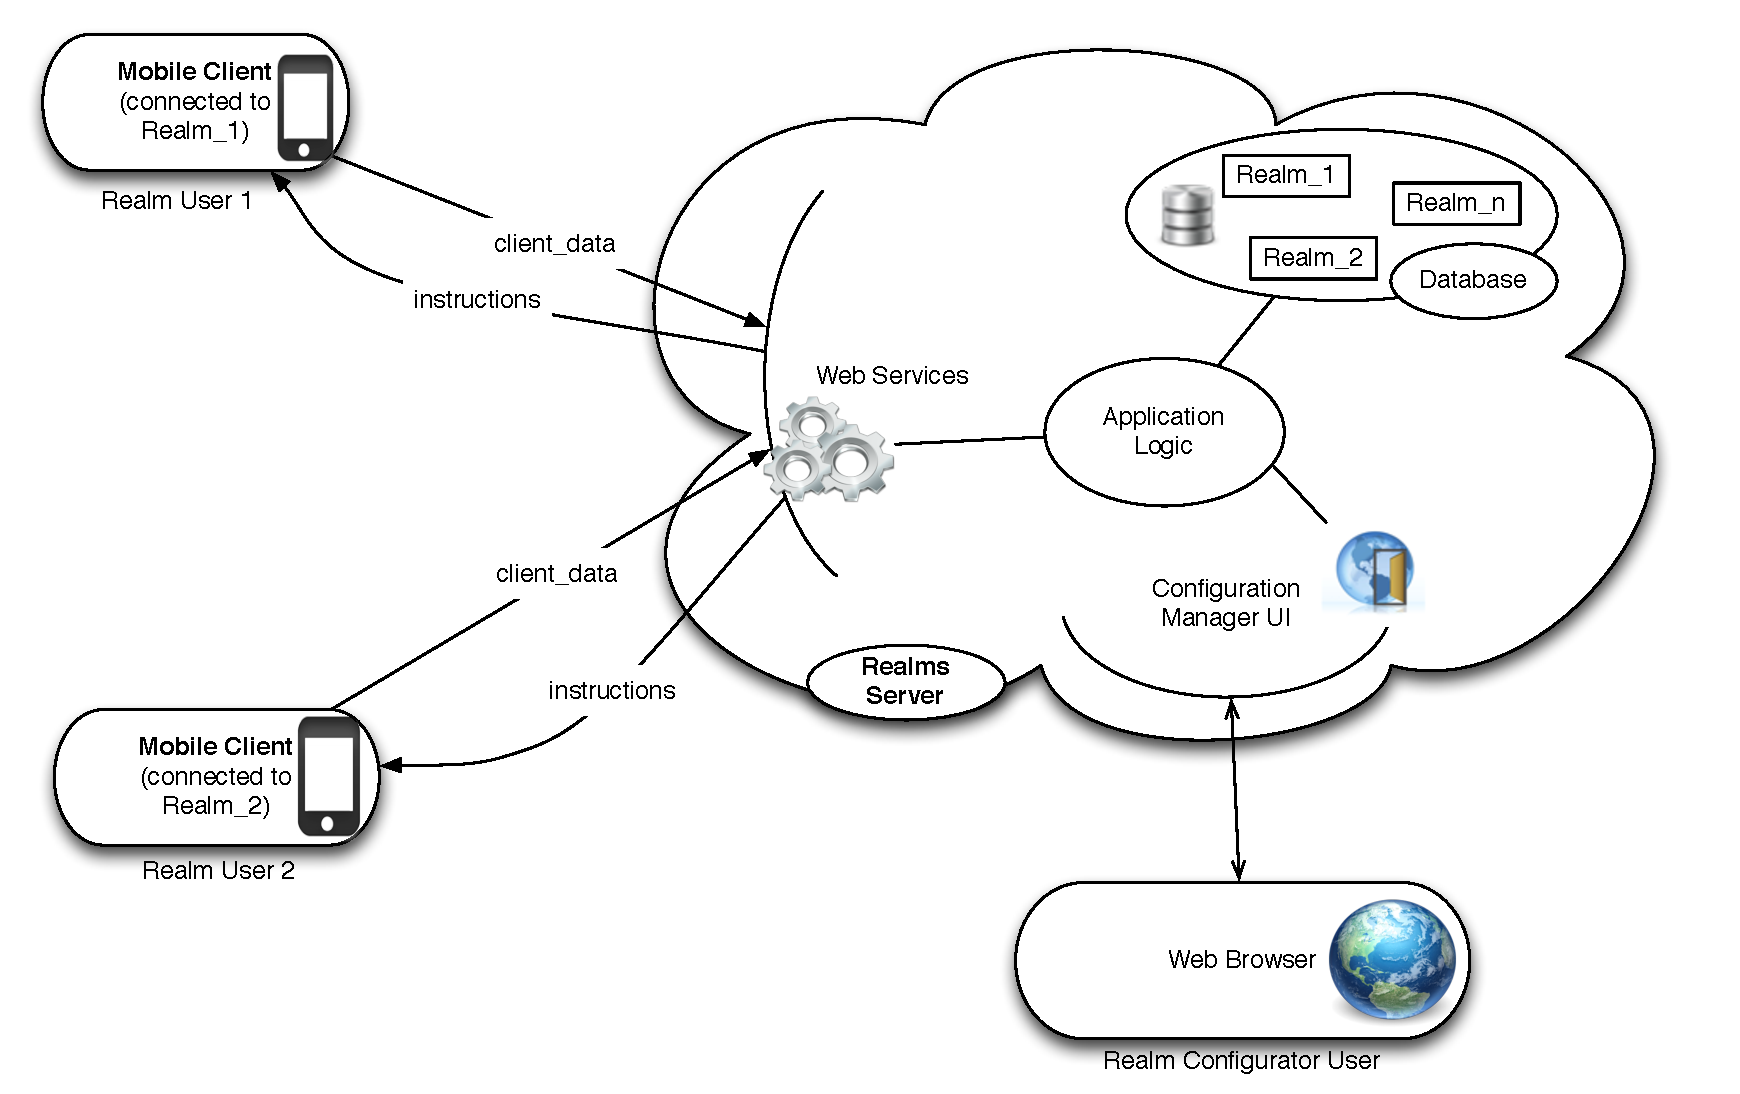
\includegraphics[width=1.0\linewidth]{fig/realms_high_lvl}
	\caption{High level system overview}
	\label{fig.design.high_lvl}
\end{figure}
\noindent Figure \ref{fig.design.high_lvl} depicts the major components and data structures of the system. The configuration manager is a standalone web application running on a stationary computer (the realms server) and is made up by the following subcomponents:
\begin{itemize}
	\item a database assuring the persistence of configured realms
	\item the application logic that holds the processing routines which take place behind the scene
	\item two interfaces to be accessed from the outside by the different clients of the system - a set of web services to be accessed by the mobile clients and a configuration UI (user interface) to be accessed by the realm configurators through a web browser. 
\end{itemize}

\noindent Before we go any further, we would like to shortly address the concrete choices we have made in the design based on the 4 dimensions identified in Section \ref{sub:taxanomy_of_location_features}:
\begin{enumerate}
	\item The location is represented in absolute values expressed in terms of latitude and longitude, which represents raw location data. In the future, this can easily be expressed as symbolic or relative applying if needed, by simply applying a few transformations on top of the raw data.
	\item For the location level have employed both levels. Location-based interactions happen when realm users receive information from the realm server based on their actual location. The realm user might be prompted to provide feedback in certain situations and the outcome of the interaction is the feedback of the user which is recorded in on the server side - this is characterised as a location-enhanced interaction.
	\item As data types, both information and commands are present. Information is the data type generated when realm users receive information based on their actual location, while providing feedback based on the current location (and associated data) is done thought a location-based command.
	\item The communication type we have employed is based exclusively on polling. That is, the user has to explicitly query the server for updates (i.e. by pressing a button).
\end{enumerate}

\noindent Figure \ref{fig.design.comm_protocol} further details the interaction between the mobile client and the server.
\\
\begin{figure}[H]
	\centering
	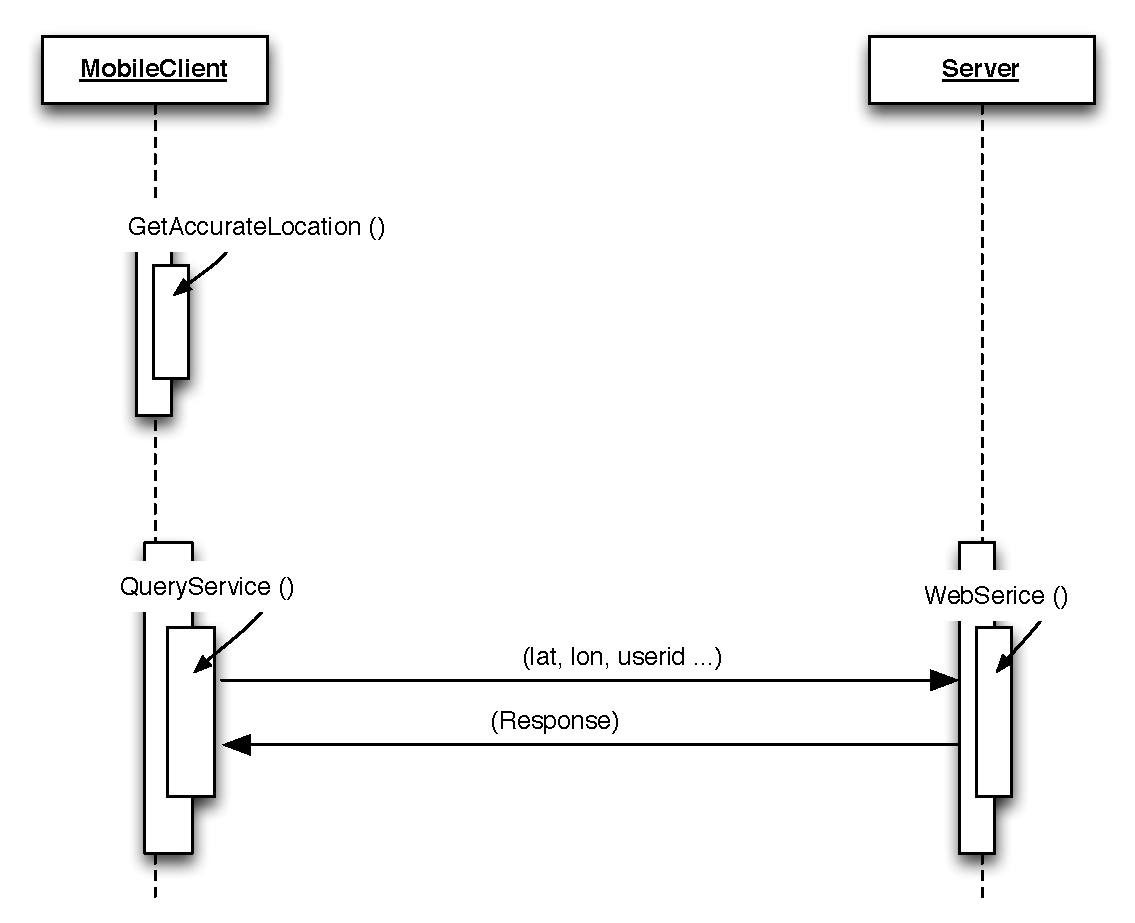
\includegraphics[width=1.0\linewidth]{fig/abstract_communication_protocol}
	\caption{Abstract Communication Protocol}
	\label{fig.design.comm_protocol}
\end{figure}
\noindent After the client is started up, it tries to communicate with the realms server sending over the authentication credentials and a realm to connect to. If the authentication is successful, the server either creates a new session or resumes and existing one; the way we manage the user sessions is an important characteristic of the system -- we are supporting long-running communication sessions between mobile phones and a server. The data connectivity of a mobile phones is still highly volatile so we have to consider as a fact that client-server communication can be broken at any time. We try to overcome this problem by storing each user session ID (and any relevant data), for each separate realm, in a persistent storage. When the mobile client starts to communicate with the server on a specific realm, the realms server will determine whether a new sessions has to be created or an existing one can be resume.
\\

\noindent Once the client got a connection to the server a series of (report status data) - (receive instructions) will follow. The client gathers location data and communicates it to the server which, using the information of the current realm, computes the instructions to be sent back to the client. The communication stops in one of the following situations: an exception occurs during the communication session, the client stops or the interaction flow got to an end.
\\

\noindent Using the term "instruction", we cover a large range of meanings that can lead to ambiguities. Instruction is the result returned by the realm server after the mobile client requested an update based on its current location. This could be a simple historical information about a of a build the user is close to, a question and a set of answers the user can choose from to provide feedback etc.
\\

\noindent Finally, as we will shortly address the concrete architecture we base our infrastructure and communication upon. As discussed by Fielding in \cite{Fielding:2000}, REST is an architecture style for distributed hypermedia systems. A web service is an API which is accessed through the HyperText Transfer Protocol (HTTP) and executed on a remote system, hosting the requested service. A RESTful web service is a web service implemented using HTTP and the principles of REST. The RESTful web service is defined by a collection of resource, each of which is defined by three main characteristics:
\begin{itemize}
  \item the base URI identifying the web service
  \item the MIME\footnote{Multipurpose Internet Mail Extensions} type of the
  data supported by the web service (JSON, XML, etc.)
  \item the web service's interface defined against the HTTP supported methods
  like POST, GET, PUT, DELETE etc.
\end{itemize}
The REST architectural style imposes a client-server architecture, which fits well our system's architecture, which is also based on a client-server approach.

\subsection{Configuration Manager} % (fold)
\label{sub:configuration_manager}
\noindent The role of the configuration manager is to present a user with an interface where location-based interactions can be defined as they should appear in the mobile app. There are two aspects when creating a realm -- on one hand there is the interface where concrete locations are augmented with virtual properties, and on the other hand there is the flow describing the interaction between a client and the server.
\\

\noindent The most intuitive interface to augment physical location is probably a virtual map which can be easily be browsed for concrete physical locations (latitude and longitude), city name, place name, address etc. These features make it easy for the user to rapidly find the desired location they want to augment. The configuration process results in a list of (location, information) pairs where location is always (latitude, longitude) and information is a simple JSON\footnote{\url{http://www.json.org}} string. The semantics of the information are interpreted in the interaction flow. In this initial implementation of the system, the information is just a list of options which is transmitted to the client and their choice is taken into consideration during the interaction flow.
\\

\begin{figure}[H]
	\centering
	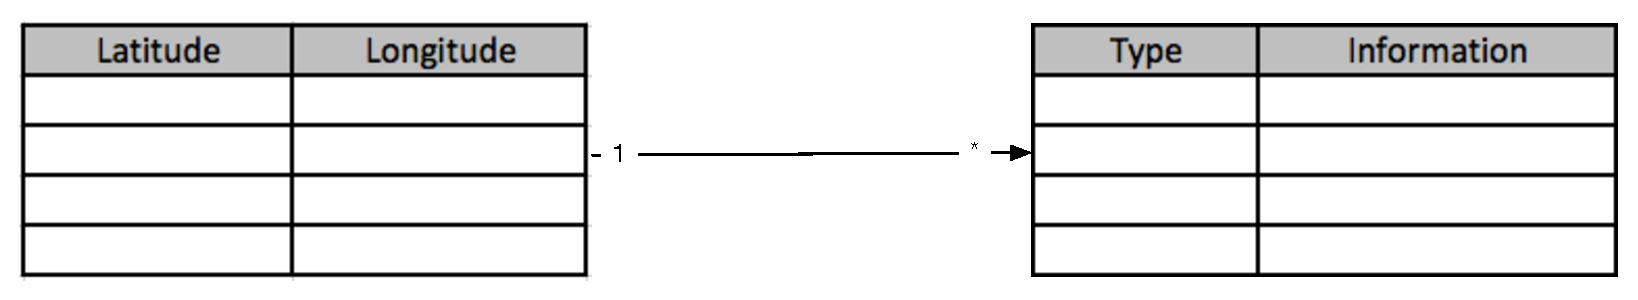
\includegraphics[width=1.0\linewidth]{fig/virtual_properties}
	\caption{Augmented Location Data}
	\label{fig.design.virtual_properties}
\end{figure}
\noindent As depicted in Figure \ref{fig.design.virtual_properties} the data will be stored in a database where concrete locations are in relation with augmented information. As the semantics of the information can be identified through their \emph{type}, this approach allows to easily enrich the types of information supported by the system in the future.
\\

In order to enable the user to easily specify the interaction flow between the client and the server we employ the workflow mechanism as it is the main mechanism to  capture and develop human-to-machine interaction \footnote{\url{http://www.interpriseo.com/resources/general_info_articles/Workflow.pdf}} consisting of a sequence of concatenated (connected) steps. Emphasis is on the flow paradigm, where each step follows the precedent without delay or gap and ends just before the subsequent step may begin. Figure \ref{fig.design.workflow} illustrates the concept of the workflow applied to our system. Each workflow has a \emph{Start} and an \emph{End} and a number of \emph{intermediate steps}. Each step of the workflow has as entry the user's current location, the optional choice of the user (based on the virtual data assigned to the user's location) and the virtual properties present at the user's location. Based in this information the step at hand will be able to decide which is the next step and when the transition will be made. 
\\

\begin{figure}[H]
	\centering
	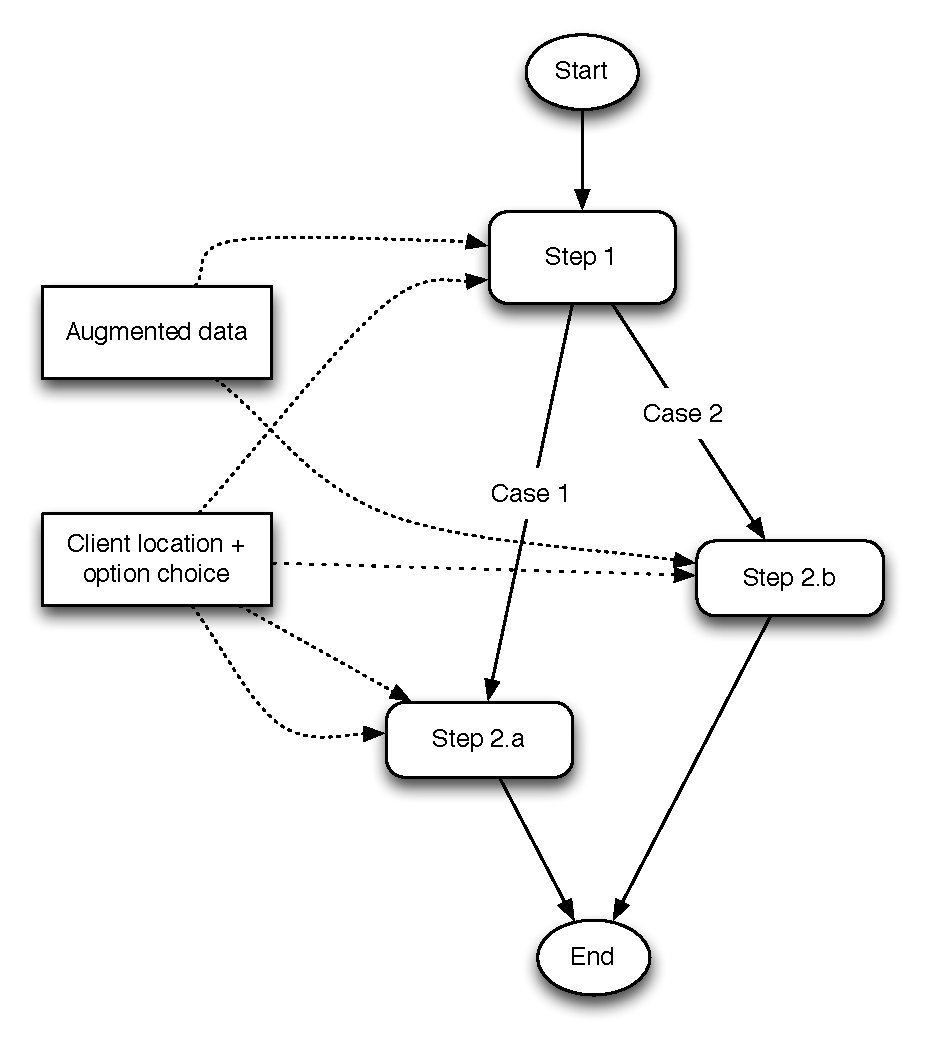
\includegraphics[width=1.0\linewidth]{fig/workflow}
	\caption{Worflow concept illustrated}
	\label{fig.design.workflow}
\end{figure}
The workflow builder is represented by a graphical tool where the user can create steps and connections inside the flow. For each step simple if-then-else decision constructs can be applied using the above mentioned variables (user location, virtual properties and optional user choice) and optional custom constants. A sketch of the tool is shown in Figure \ref{fig.design.workflow_sketch}.
\begin{figure}[H]
	\centering
	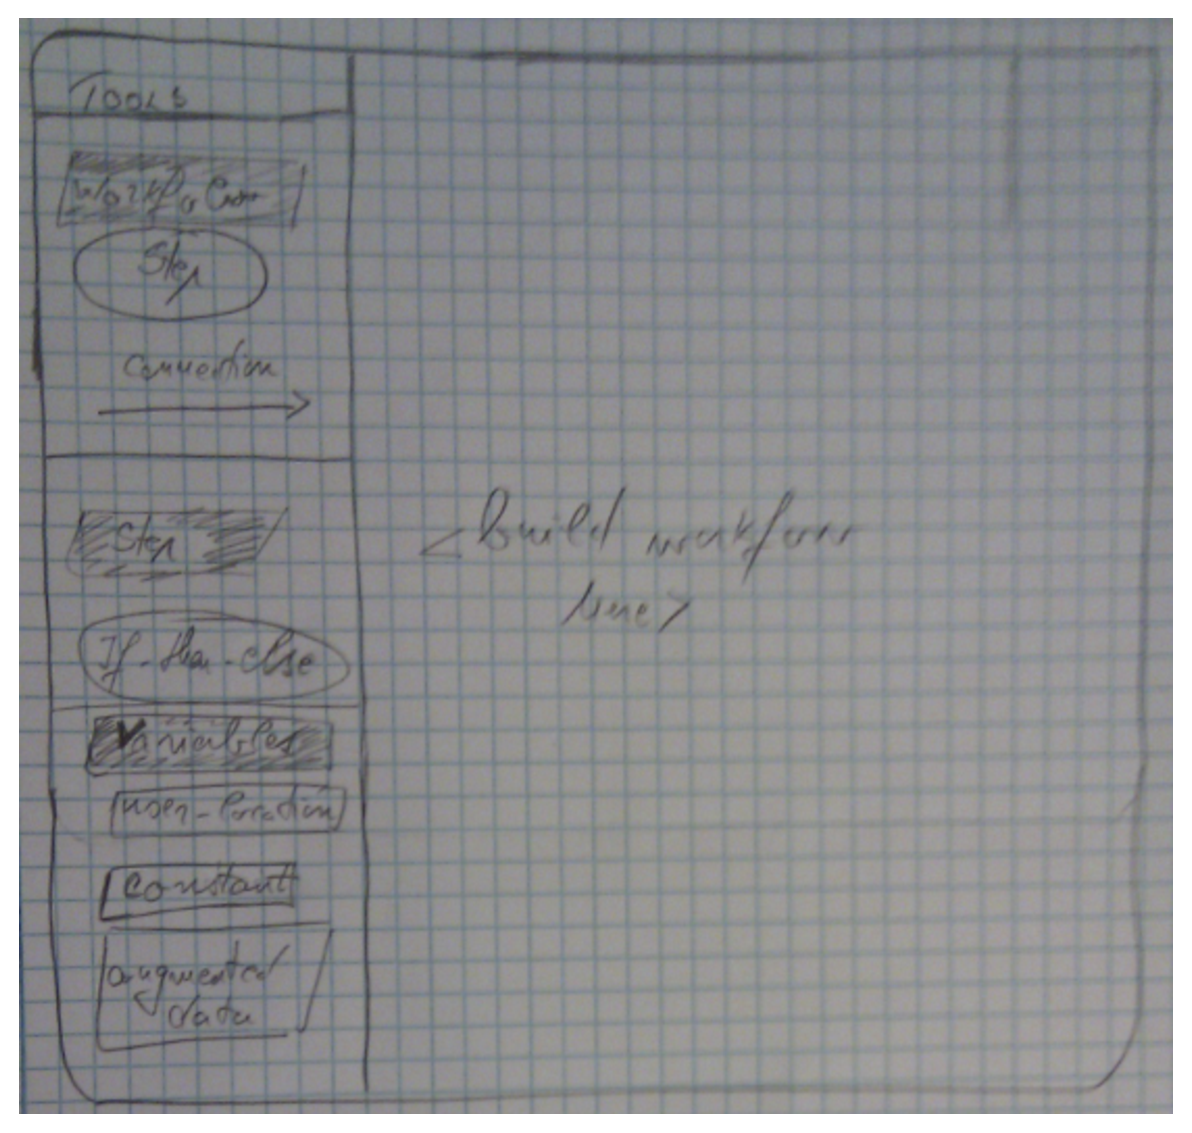
\includegraphics[width=0.9\linewidth]{fig/workflow_sketch}
	\caption{Worflow tool UI sketch}
	\label{fig.design.workflow_sketch}
\end{figure}
\\

For the current prototype we omitted this feature as it introduces a high level of complexity. Instead, we created a fixed interaction scenario -- "The realm user requests an update based on the current location. The realms server receives the request and computes the nearest virtual information, based on the location information, in the current realm which is returned to the mobile client which can provide a feedback". In short, we have implemented a workflow based on the request-reply programming model \cite{Coulouris:2005}.
% subsection configuration_manager (end)be available having 

\subsection{Realms Android App} % (fold)
\label{sub:realms_android_app}
The mobile application presents users with the ability to access realms and interact with them as described by their configuration. It is also meant to collect location information which is a required piece of data needed by the server to successfully guide the user through the realm's workflow. Figure \ref{fig.design.mobile_client} depicts the main data structures and the interface the mobile client should implement to communicate with the realms server.
\begin{figure}[H]
	\centering
	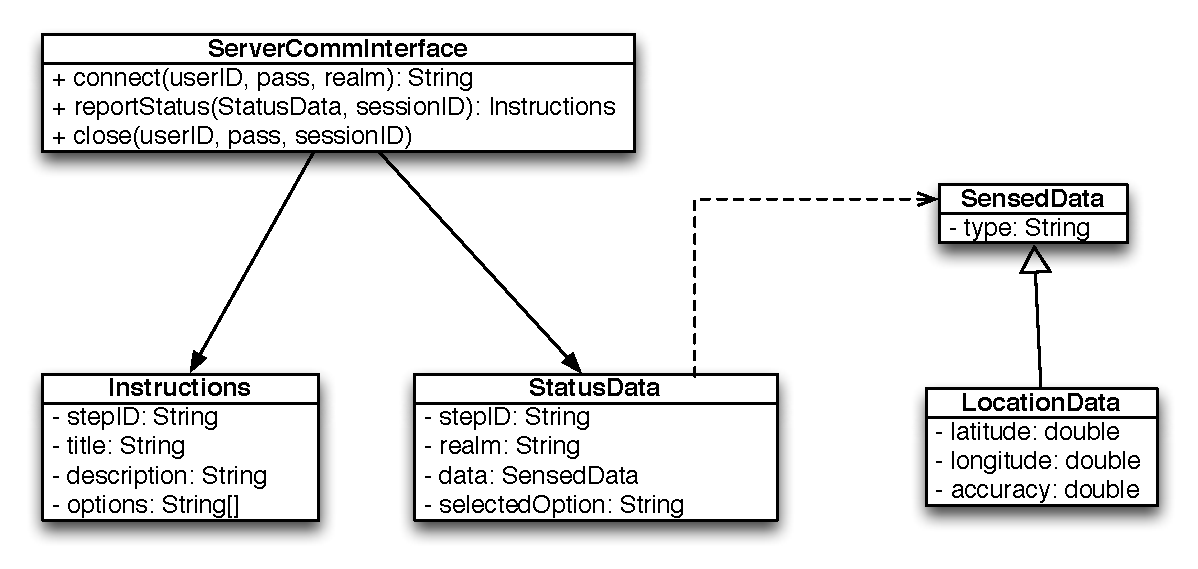
\includegraphics[width=1.0\linewidth]{fig/mobile_client}
	\caption{Data structures and communication interface which allows the mobile client to communicate with the realms server}
	\label{fig.design.mobile_client}
\end{figure}
% subsection realms_android_app (end)
% section design (end)

\subsection{Realms Infrastructure} % (fold)
\label{sub:realms_infrastructure}
The realms infrastructure is the central component of our system and handles connections from the mobile app and the configuration manager, and stores information such as location-based information and configurations. Although we do not follow any cloud computing standards, we look at our infrastructure as described by the \emph{cloud computing} paradigm: it offers services to clients which must meet one constraints: provide the service accurately with the require data (i.e. location data). Basically, with this approach we hold the data and the computation in the \emph{realms cloud}, hence the clients only need to provide the service with the required data and present the users with the results from the services.
\\\\
The infrastructure provide a RESTful API with the following methods:
\begin{itemize}
	\item \emph{connect(userID, pass, realm)} -- try to authenticate a client based on the submitted credentials for the specified realm; it the authentication was successful, determine whether the user is already in a session which needs to be resumed. If so, return the existing sessionID, otherwise create a new session and start processing processing the realm's flow from the first step (for this user)
	\item \emph{reportStatus(StatusData, sessionID)} -- receive status data from the client. Process the current step and advance in the flow, if the all the conditions imposed by the current step are met, and return the client with a new set of \emph{instructions}
	\item \emph{close(userID, pass, sessionID, realm)} -- force end the current session (even if the flow is not finished)
\end{itemize}
% subsection realms_infrastructure (end)